\section{Tools and Scenario Installation}
\label{sec:install}

After describing the tools used, we now move to the setup of what is needed to reproduce the project. All the configuration files and codes can be found in a GitHub repository\footnote{\url{https://github.com/Soldera21/k8s-detection-response}}. The requirements are the following:
\begin{itemize}
    \item \textbf{Minikube} as local environment or a \textbf{Kubernetes} cluster;
    \item \textbf{kubectl} to interact with Kubernetes;
    \item \textbf{Helm} for package management;
    \item \textbf{Docker} for building and managing container images;
    \item \textbf{virtualization engine} depending on the OS.
\end{itemize}
Installation guide of all the tools can be found at the following links: Minikube\footnote{\url{https://minikube.sigs.k8s.io/docs/start/}}, kubectl\footnote{\url{https://kubernetes.io/docs/tasks/tools/}}, Helm\footnote{\url{https://helm.sh/docs/intro/install/}}, Docker\footnote{\url{https://docs.docker.com/engine/install/}}.
We used Minikube in our local machine. Before running anything we need to start it using \texttt{minikube start}. If it is the first time running Minikube it will take longer because of image download and setup. Every time we do \texttt{minikube stop} it will pause the virtual machine of Minikube, permitting to resume it where we left. Minikube supports also multiple virtualization engines based on the host OS used like Docker, VirtualBox, VMWare, HyperV and many others.

For every tool and scenario we prepared a set of scripts included in the repository to setup, start and stop every resource needed. There should not be problems running Falco and Tracee at the same time or to mix some scenarios, but we suggest to run one scenario and one detection tool at a time to be able to get clear results.

All the scripts used to build images are made for Linux. In Windows alternative commands can be used and they are commented inside the building scripts.


\subsection{Falco}
The installation of Falco is done adding the Falcosecurity Repository. Then Helm is used to deploy the application in the cluster. The setup we used also includes Falco Sidekick to send events to an external entity. All the configuration files for Falco startup and Sidekick are in the folder \texttt{falco-conf/falco-rules}. In our case we made an event handler in Python that is able to receive JSON data through a webhook and parse it to apply some automatic countermeasures in the cluster (we labeled the deployment that triggered the alert, but actions such as scaling the deploymentnto 0 replicas can be taken). First of all we need to build the image that is in \texttt{falco-conf/falco-handler}. Then we can start also the handler pod with its related service. It requires a set of permissions on the cluster that can be found in \texttt{falco-conf/manifests/falco-handler-rbac.yaml} to find pods that are causing alerts and to edit the respective deployments. In particular we are creating a service account for the handler and we are associating it to a role with capabilities on pods and deployments of the entire cluster, regardless of the namespace. The main challenge of the handler is to extract pod, deployment and namespace name from the event. In Falco we added also a custom rule preventing alerts from the event handler that can be triggered when it uses K8s API to perform actions in the cluster. It can be found in \texttt{falco-conf/falco-rules/custom-rules.yaml}.\\
The following commands need to be run from the root folder of the project to start Falco and its handler:
\begin{enumerate}
    \item \textbf{Install and start Falco}:\\
    \texttt{bash falco-conf/falco-install.sh}
    \item \textbf{Build handler image}:\\
    \texttt{bash falco-conf/falco-handler-build.sh}
    \item \textbf{Start handler}:\\
    \texttt{bash falco-conf/falco-handler-start.sh}
\end{enumerate}
Now doing \texttt{kubectl get pods -A} we have to check that Falco, Falco Sidekick and Falco handler pods are in "Running" state.\\
This can be stopped doing:
\begin{enumerate}
    \item \textbf{Stop Falco}:\\
    \texttt{bash falco-conf/falco-remove.sh}
    \item \textbf{Stop handler}:\\
    \texttt{bash falco-conf/falco-handler-stop.sh}
\end{enumerate}


\subsection{Tracee}
To install Tracee we have to add the Aqua Security repository. Like for Falco, we deploy Tracee using Helm. After installing this tool we have to patch the DaemonSet to configure it to send events also to the webhook using the file \texttt{tracee-conf/tracee-rules/tracee-ds-patch.yaml}. All the other mechanisms are the same as those used in Falco with the event handler with permissions that is receiving events. The only difference is in the handler code because events form Tracee don't contain the pod's namespace. We need to query the cluster using \texttt{kubectl} to retrieve the namespace and then apply automatic actions. Tracee doesn't have any problem when the handler is contacting K8s API so we don't need any additional rule.\\
The following commands need to be run from the root folder of the project to start Tracee and its handler:
\begin{enumerate}
    \item \textbf{Install and start Tracee}:\\
    \texttt{bash tracee-conf/tracee-install.sh}
    \item \textbf{Build handler image}:\\
    \texttt{bash tracee-conf/tracee-handler-build.sh}
    \item \textbf{Start handler}:\\
    \texttt{bash tracee-conf/tracee-handler-start.sh}
\end{enumerate}
Now doing \texttt{kubectl get pods -A} we have to check that Tracee, Tracee operator and Tracee handler pods are in "Running" state.\\
This can be stopped doing:
\begin{enumerate}
    \item \textbf{Stop Tracee}:\\
    \texttt{bash tracee-conf/tracee-remove.sh}
    \item \textbf{Stop handler}:\\
    \texttt{bash tracee-conf/tracee-handler-stop.sh}
\end{enumerate}


\subsection{Scenario: ZipApp}
We implemented a web application called \textbf{ZipApp} in order to simulate realistic attack scenarios and test our runtime threat detection tools. The script used was inspired by a challenge originally developed for CyberChallenge, which was adapted to suit the goals of our project.\\
This web application is intentionally insecure and its key vulnerability is its improper handling of uploaded file names and paths. Specifically, it does not validate or sanitize user-supplied filenames when serving files for download in zipped form.

The image is built with all the necessary tools installed inside and the script of the server. To launch build for Minikube environment we use:

\texttt{bash scenario/zipapp-build-images.sh}

\noindent This will build images for every scenario we will present later. In particular we will discuss about the particular vulnerability exploited, the attacks performed and the possible countermeasures in the next sections. A basic and vulnerable version can be started using:

\texttt{bash scenario/zipapp-normal-start.sh}

\noindent and removed with:

\texttt{bash scenario/zipapp-nor-sec-remove.sh}

When the application deployment is started with its service, we can copy the URL provided by Minikube and connect to the website using a browser. What we can see is shown in \autoref{fig:login} and we can login with whatever credentials (no verification, only for example purpose).

\begin{figure}[H]
    \centering
    \fbox{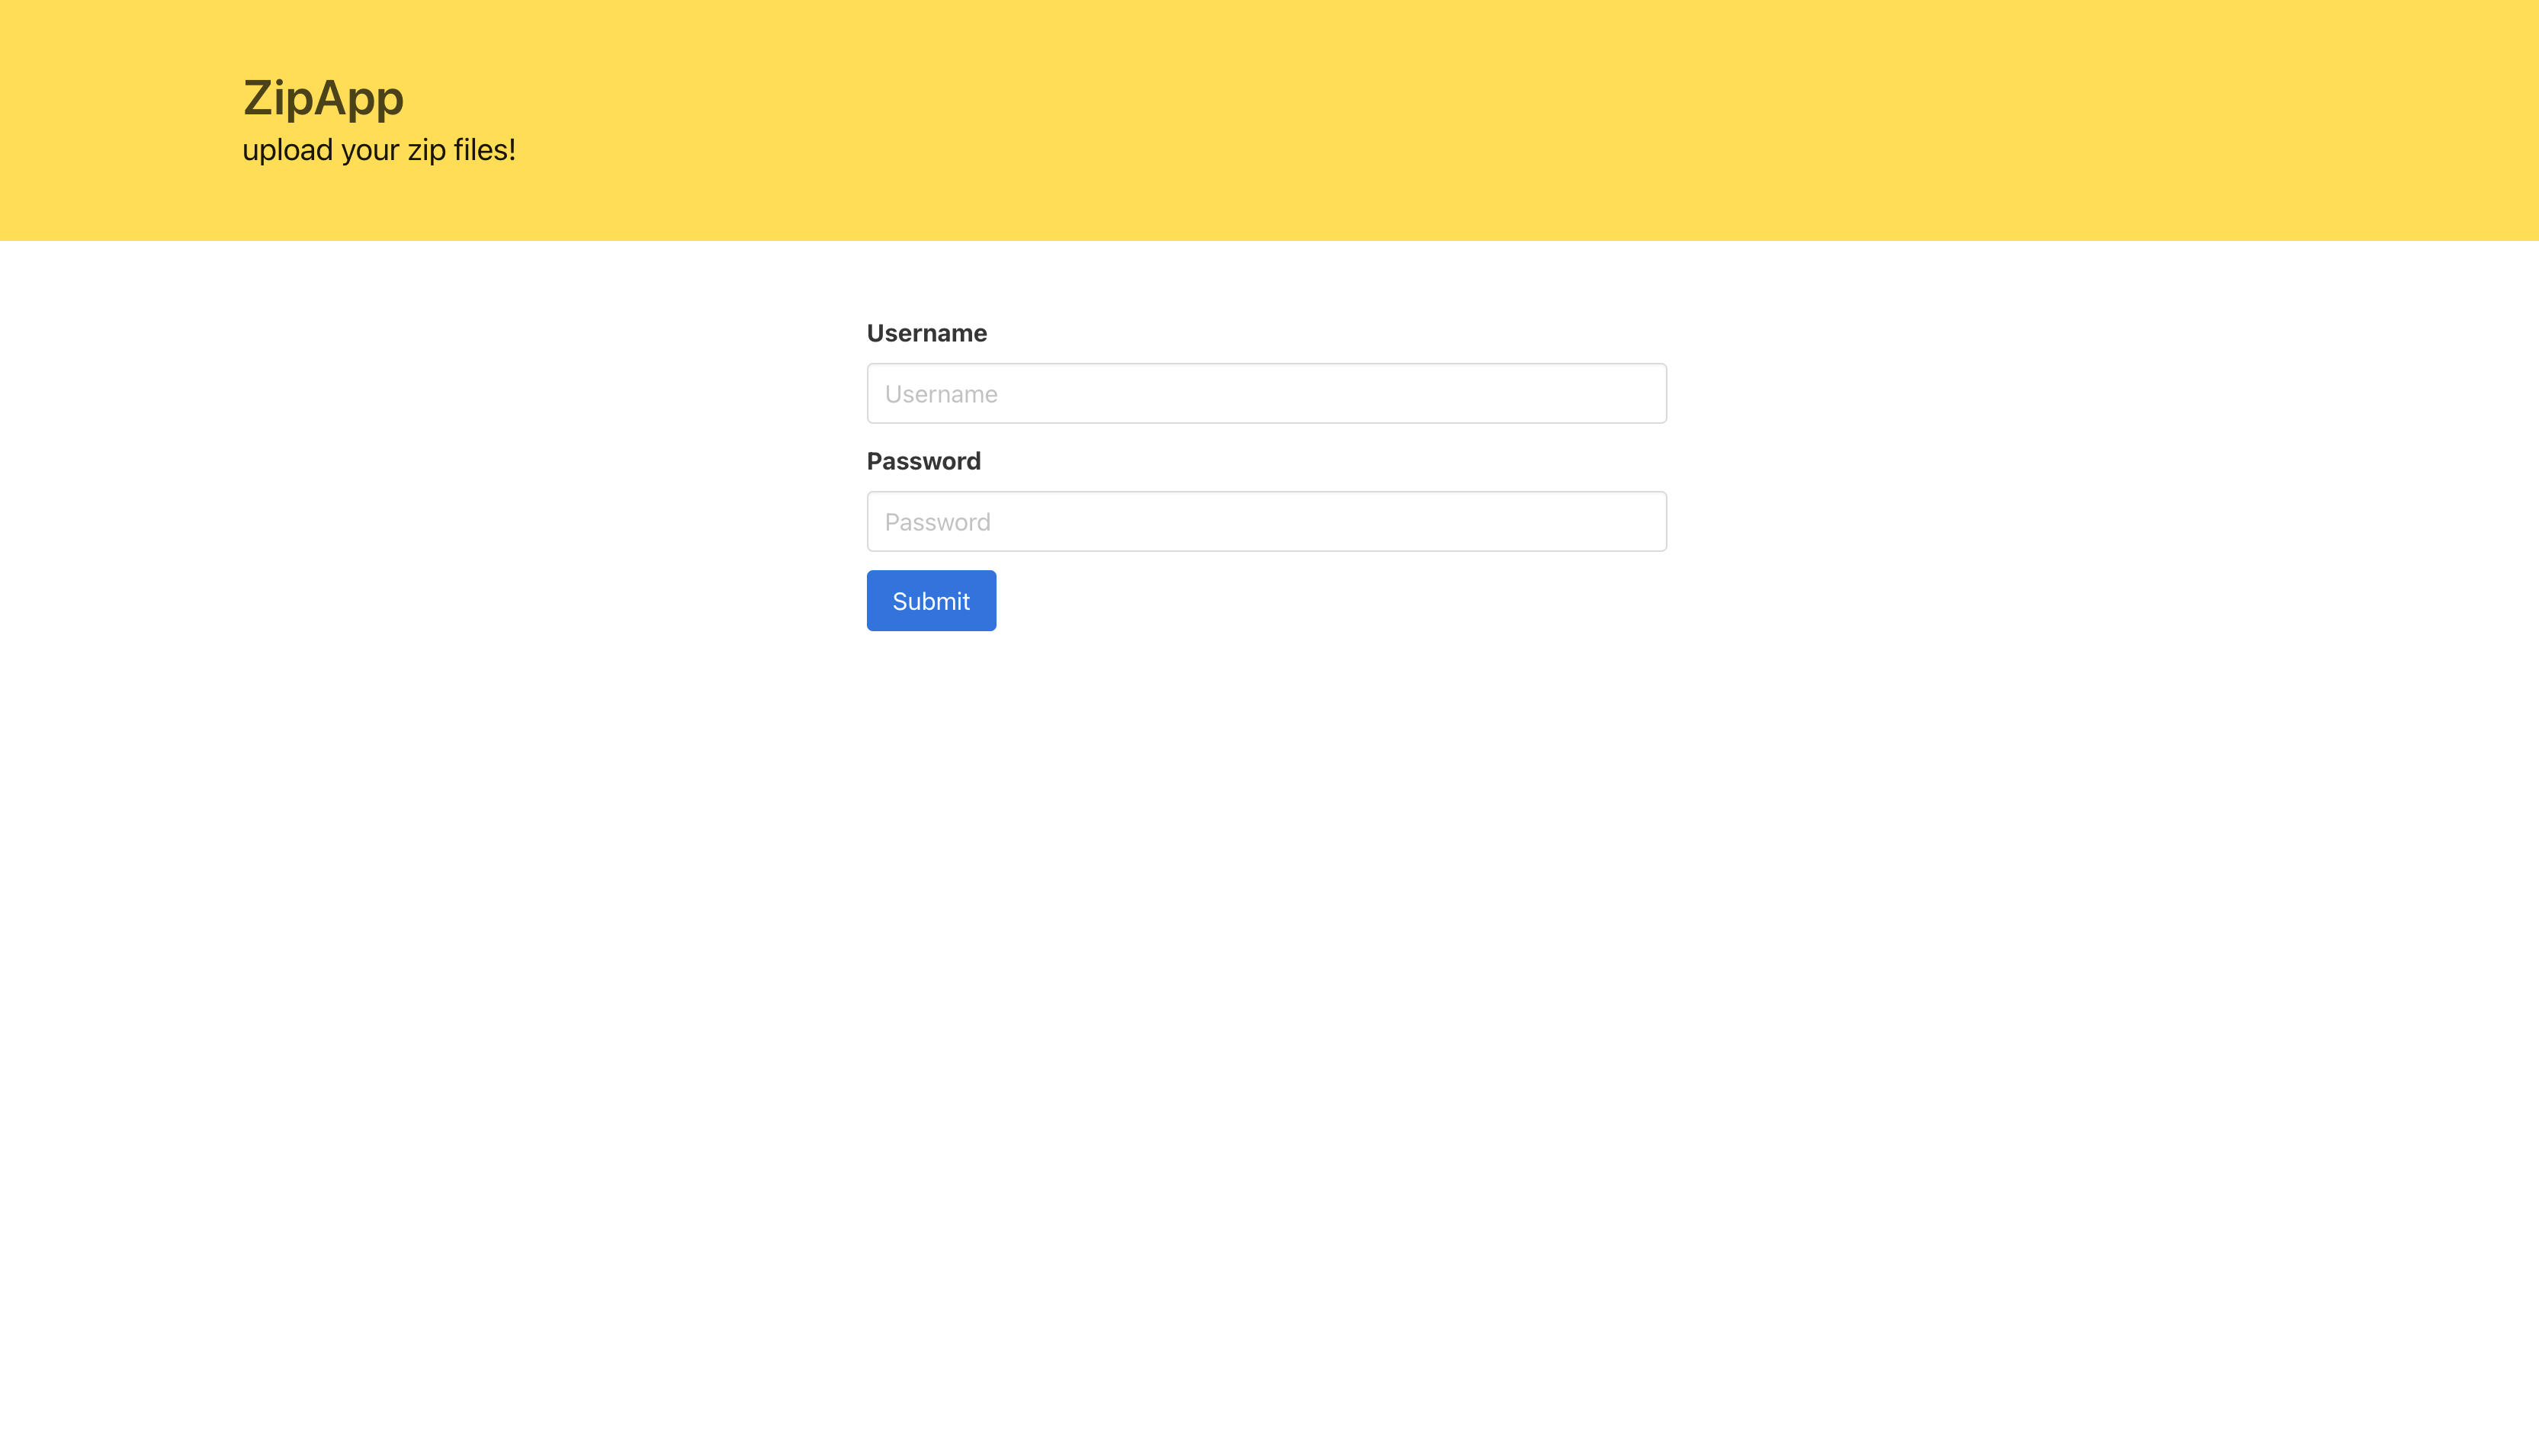
\includegraphics[width=0.70\linewidth]{images/login.png}}
    \caption{Login Screen of the Example WebApp}
    \label{fig:login}
\end{figure}

After logging we have another screen shown in \autoref{fig:nofiles} where we can upload a new zip to add files to the pool of the current logged user. All these data is saved inside \texttt{/tmp} folder and every user has a token that names a folder associated.

\begin{figure}[H]
    \centering
    \fbox{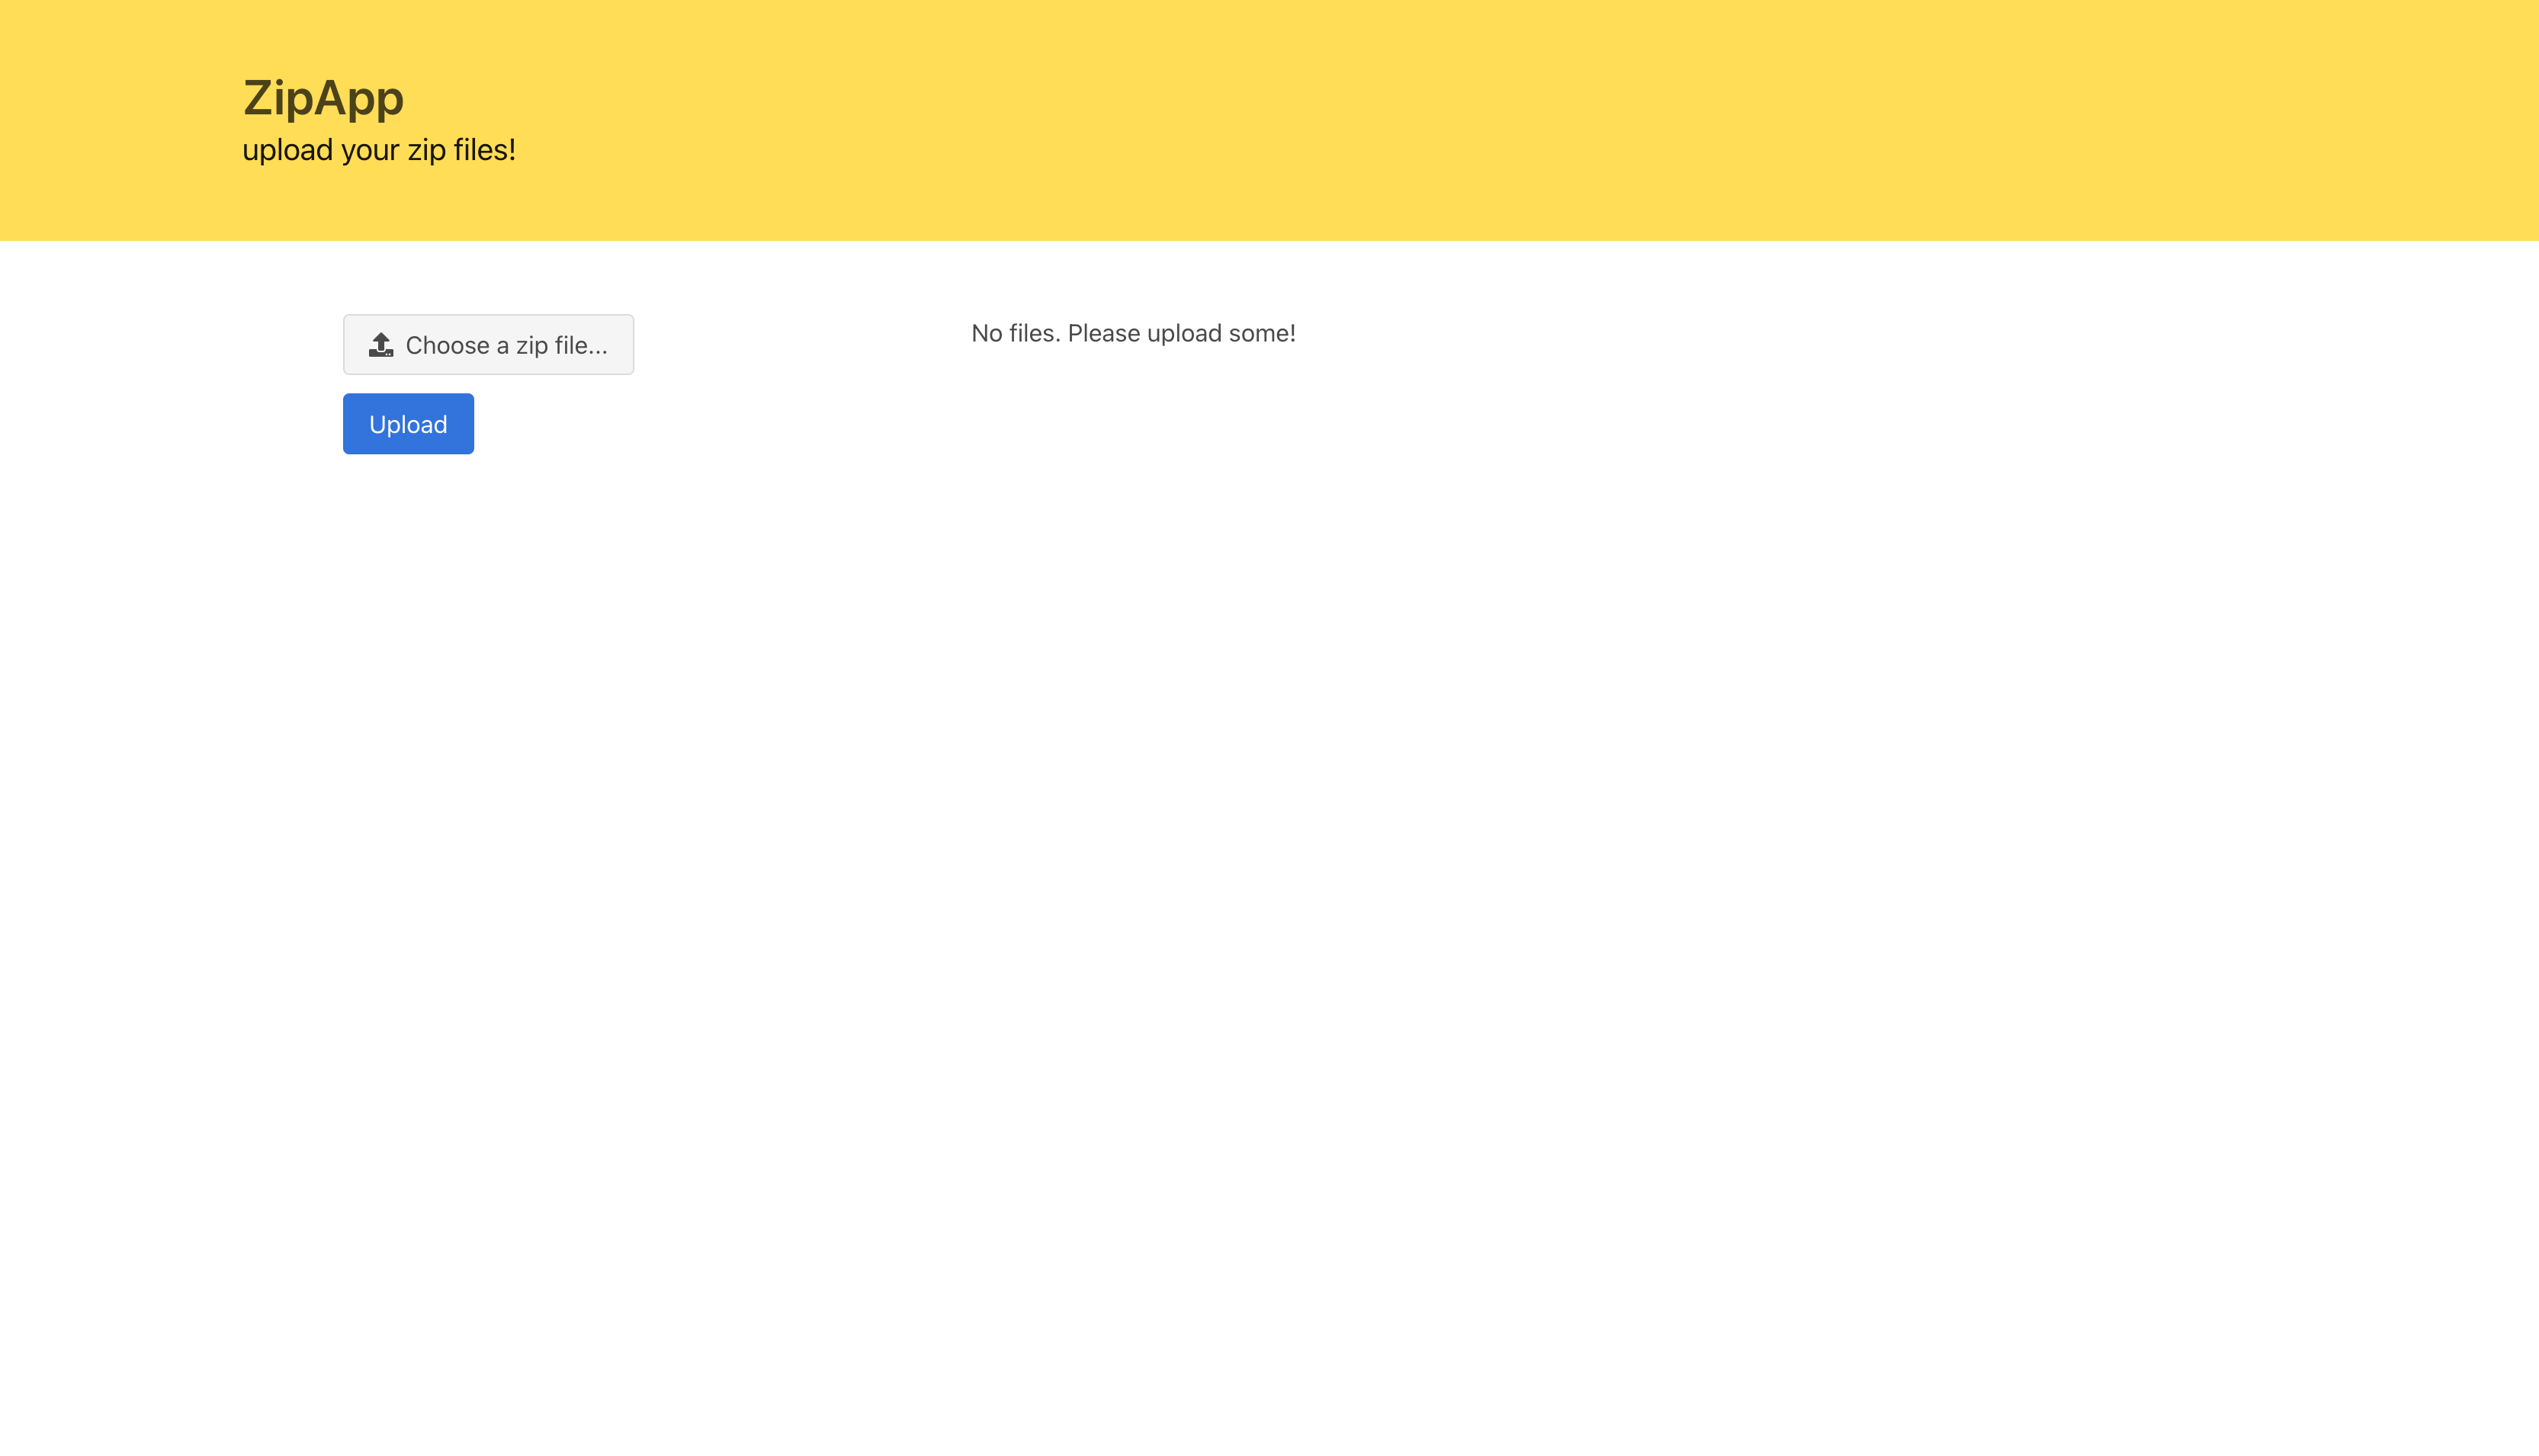
\includegraphics[width=0.70\linewidth]{images/nofiles.png}}
    \caption{Upload Screen of the Example WebApp}
    \label{fig:nofiles}
\end{figure}

Finally when files are uploaded, they can be downloaded either as a new zip or individually by clicking on them. We can also upload a new zip to add other files to the pool. This is show in \autoref{fig:uploaded}.

\begin{figure}[H]
    \centering
    \fbox{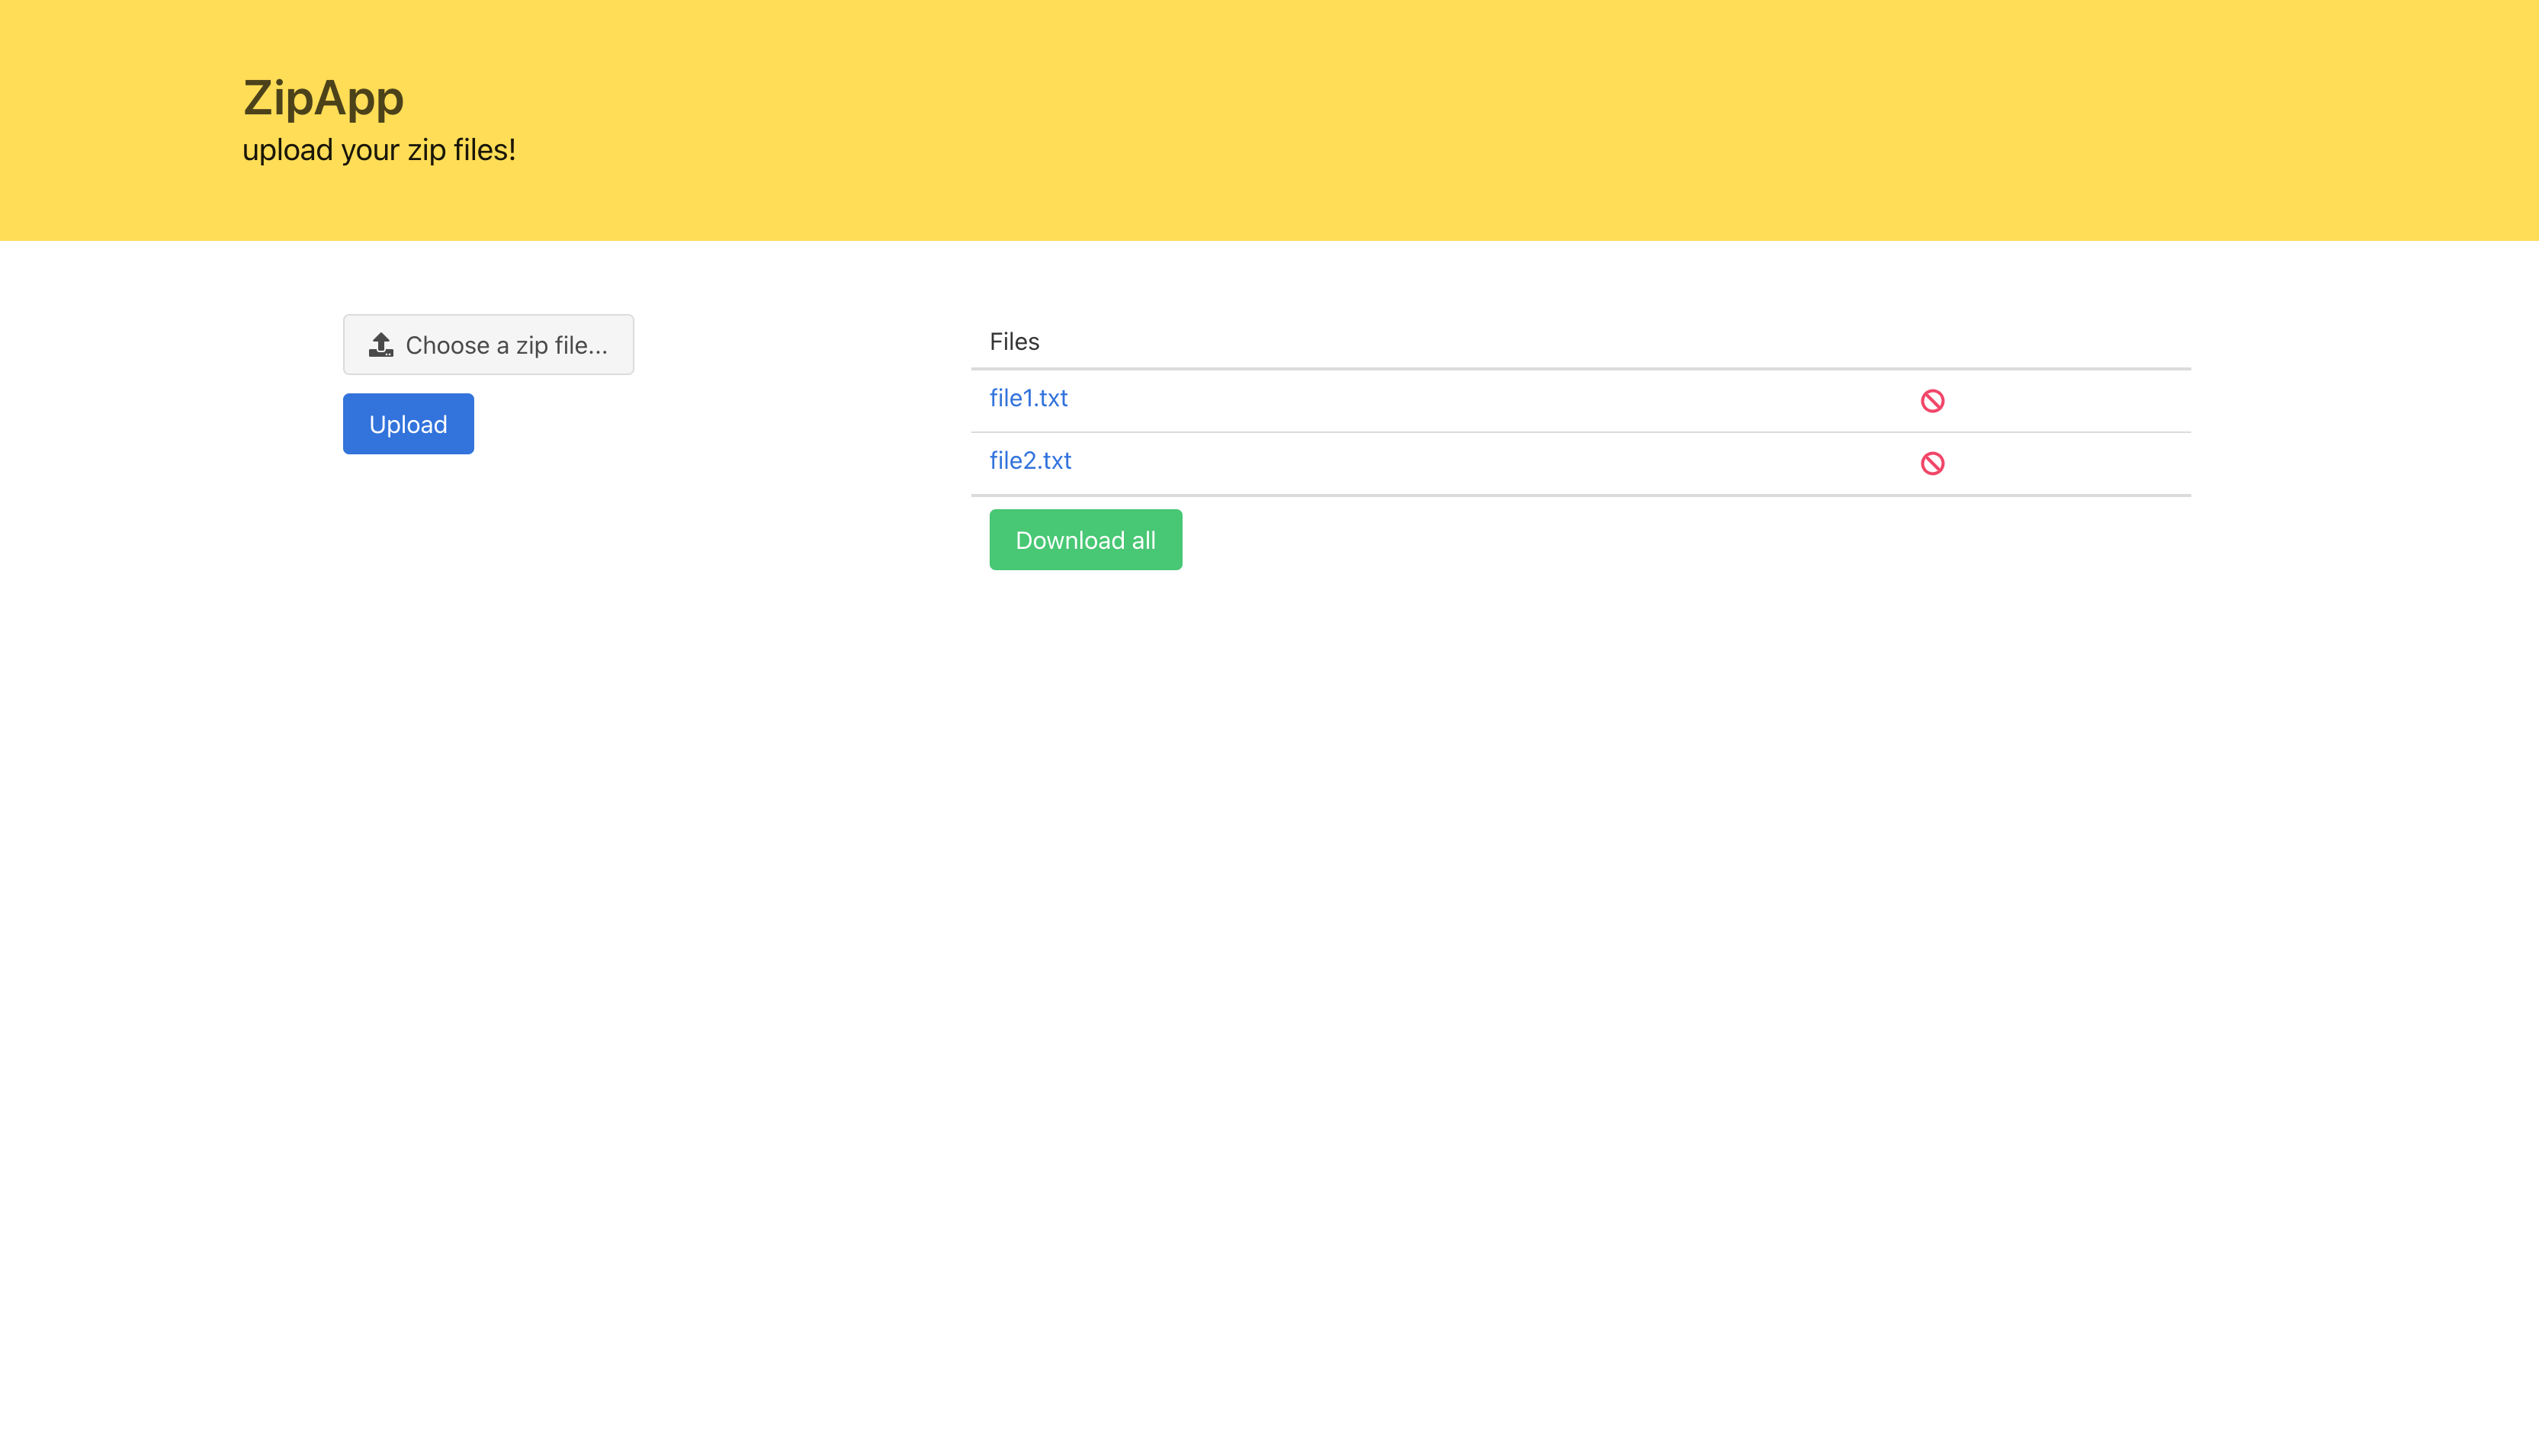
\includegraphics[width=0.70\linewidth]{images/uploaded.png}}
    \caption{Screen of the Example WebApp with some Uploaded Files}
    \label{fig:uploaded}
\end{figure}

